\subsection{Constructive resolution and a continuum action}
\label{sec:indexed-leakage-action}

The preceding monic identification makes the unresolved mode budget a
weighted polynomial approximation problem. It also permits a sufficient
indexed bound that does not mistake a signed orthogonality identity for
a positive error estimate.

\begin{proposition}[Cardinal-subspace resolution bound]
\label{prop:cardinal-resolution}
Assume the positive real atomic measure of the preceding subsection,
with distinct ordered positive-weight atoms $t_i$ and weights $\mu_i$.
Let $\theta_k$ be its degree-$N$ zero-shift Ritz root. Choose $k\leq N$
polynomials $q_i$ of degree at most $N-1$ with
$q_i(t_j)=\delta_{ij}$ for $1\leq i,j\leq k$. Put
\[
 D_k=\operatorname{diag}(\mu_1,\ldots,\mu_k),\qquad
 E_k=\sum_{m>k}(t_m-t_k)\mu_m q(t_m)q(t_m)^T,
 \qquad B_k=\operatorname{tr}(D_k^{-1}E_k).
\]
Then $0\leq\theta_k-t_k\leq B_k$. In particular, $d$ relative digits
for the zero-shift ordinate are guaranteed if
\[
 N\geq k,\qquad B_k\leq t_k\bigl(2\,10^{-d}+10^{-2d}\bigr).
\]
\end{proposition}
\begin{proof}
The cardinal evaluations make the chosen trial space $k$-dimensional.
For $q_c=\sum_i c_iq_i$, its norm squared is at least $c^TD_kc$, while
its energy relative to $t_k$ is at most $c^TE_kc$: the first $k$ atoms
contribute $\sum_i\mu_i(t_i-t_k)c_i^2\leq0$. Min--max therefore bounds
$\theta_k-t_k$ by the largest eigenvalue of
$D_k^{-1/2}E_kD_k^{-1/2}$, hence by its trace since it is positive
semidefinite. The lower bound is the full multiplication-operator
min--max bound. Finally the relative ordinate error is at most
$\sqrt{1+B_k/t_k}-1$, which gives the stated digit threshold.
\end{proof}

This bound needs only finite moments once the cardinals are supplied.
If $U$ contains their coefficients in the polynomial basis of the
moment pair $(T,H)$, then exactly
\[
 E_k=U^T(T-t_kH)U-\operatorname{diag}\bigl(\mu_i(t_i-t_k)\bigr).
\]
For example, cardinal polynomials on the first $M$ atoms, $k\leq M\leq N$,
also remove atoms $k+1,\ldots,M$. All 3311 exact rational checks on
119 finite positive-measure fixtures pass. The bound is conditional on
the stated measure, and evaluating it currently uses reference atoms;
it is not yet an explicit $C,N,k$ estimate. A failed upper bound is
inconclusive, whereas $N<k$ cannot represent a complete movable prefix.
The ground-energy shift and the $P$-dependent arithmetic channel must
still be added before applying the earlier soft minimum.

\paragraph{A model with an explicit mode-dependent turning point.}
The rational-Ritz potential approach\cite{BGV2010} suggests retaining
the finite Fourier lattice in a continuous approximation. Write
$L=\log C$ and $A=2\pi N/L$. Replace its pole density by
$L\mathbf1_{|x|<A}/(2\pi)$ and the zeta atoms by the smooth density
$\log(|x|/(2\pi))/(2\pi)$. These replacements discard discreteness
and the exact sine carrier. The latter density is even negative for
$|x|<2\pi$, so this is a formal logarithmic-defect model, not a proved
positive equilibrium measure at the origin.

Solving the corresponding finite Hilbert-transform problem with
potential zero outside $[-a,a]$ and no square-root endpoint term gives
\begin{equation}\label{eq:action-endpoint}
 \log\frac{a}{4\pi}=\frac{2L}{\pi}
       \arcsin\!\left(\min\left\{\frac{A}{a},1\right\}\right).
\end{equation}
Thus $a=4\pi C$ when $N\geq2C\log C$; otherwise there is a unique
solution $a>A$. This is a model transition, not an established CCM
resolution threshold. For $4\pi<x<4\pi C$, inversion gives
\begin{equation}\label{eq:action-mode-threshold}
 N_{\mathrm{turn}}(C,x)=\frac{x\log C}{2\pi}
       \sin\!\left(\frac{\pi\log(x/(4\pi))}{2\log C}\right).
\end{equation}
Setting $x=\gamma_k$ exposes the indexed requirement; the separate
degree bound $N\geq k$ remains necessary for a complete movable prefix.

For $0\leq x<a$, let $s=\sqrt{a^2-x^2}$. In the mode-limited case
$A<a$, put $b=\sqrt{a^2-A^2}$. The candidate leading exponent is
\begin{align}
 \mathcal S_{C,N}(x)&=s-x\arccos(x/a)+\frac L\pi I(x),
       \label{eq:finite-mode-action}\\
 I(x)&=A\log\left|\frac{s+b}{s-b}\right|
       -x\log\left|\frac{As+bx}{As-bx}\right|.\nonumber
\end{align}
The apparent singularities cancel at $x=A$, where
$I(A)=2A\log(a/A)$. When $A\geq a$, omit $I$. In particular,
$\mathcal S_{C,N}(0)=a+4N\operatorname{arcosh}(a/A)$ in the
mode-limited regime and $4\pi C$ otherwise. Independent differentiation,
quadrature, Hilbert-transform and edge-limit evaluations pass 38
high-precision point checks; these are formula checks, not interval
certificates of a CCM approximation.

\paragraph{An unfitted test and its limitations.}
The exploratory prediction $D_k=\mathcal S_{C,N}(\gamma_k)/\log10$
uses no fitted constants. Table~\ref{tab:continuum-action-test} compares
it only on the counted, reference-window-matched point-state prefixes
inside its domain. All 5000 requested rows are retained, including the
two valid $N=750$ targets outside the modeled turning point and every
unresolved source target. The model's extra two $N=1000$ windows are
not valid indexed measurements and do not enter its score.

\begin{table}[htbp]
\centering\small
\begin{tabular}{rr|rr|rr}
\toprule
$C$ & $N$ & Counted prefix & Model prefix$^*$ & RMS digits & 1\% passes\\
\midrule
125 &1500 &$\geq1000$ &$\geq1000$ &2.1482 &4/1000\\
250 &750  &578 &576 &2.4308 &0/576\\
250 &1000 &797 &799 &2.4457 &0/797\\
250 &1250 &$\geq1000$ &$\geq1000$ &2.3131 &0/1000\\
250 &1500 &$\geq1000$ &$\geq1000$ &2.0765 &1/1000\\
\bottomrule
\end{tabular}
\caption{Leading continuum action against stored point-state root errors.
The RMS measures error in relative decimal depth; the stricter final
column tests relative displacement error below 1\%. $^*$Only the first
1000 reference ordinates are counted for the model.}
\label{tab:continuum-action-test}
\end{table}

The mode-dependent endpoint lies within two ordinates of both observed
prefix boundaries. At $C=250,N=1500$ it reduces the bare cutoff action's
189.33-digit RMS discrepancy to 2.08 digits. Nevertheless, only 5 of the
4373 eligible comparisons pass the displacement gate: the action is
\emph{not} an accurate final error formula. Its root-specific prefactor,
discrete carrier effects, transfer from the zero-shift measure to the
ground source, uniform remainder and arithmetic budget remain open.
Neither a fitted correction nor a clipped zero-digit claim is added.
\begin{figure}[htbp]
\centering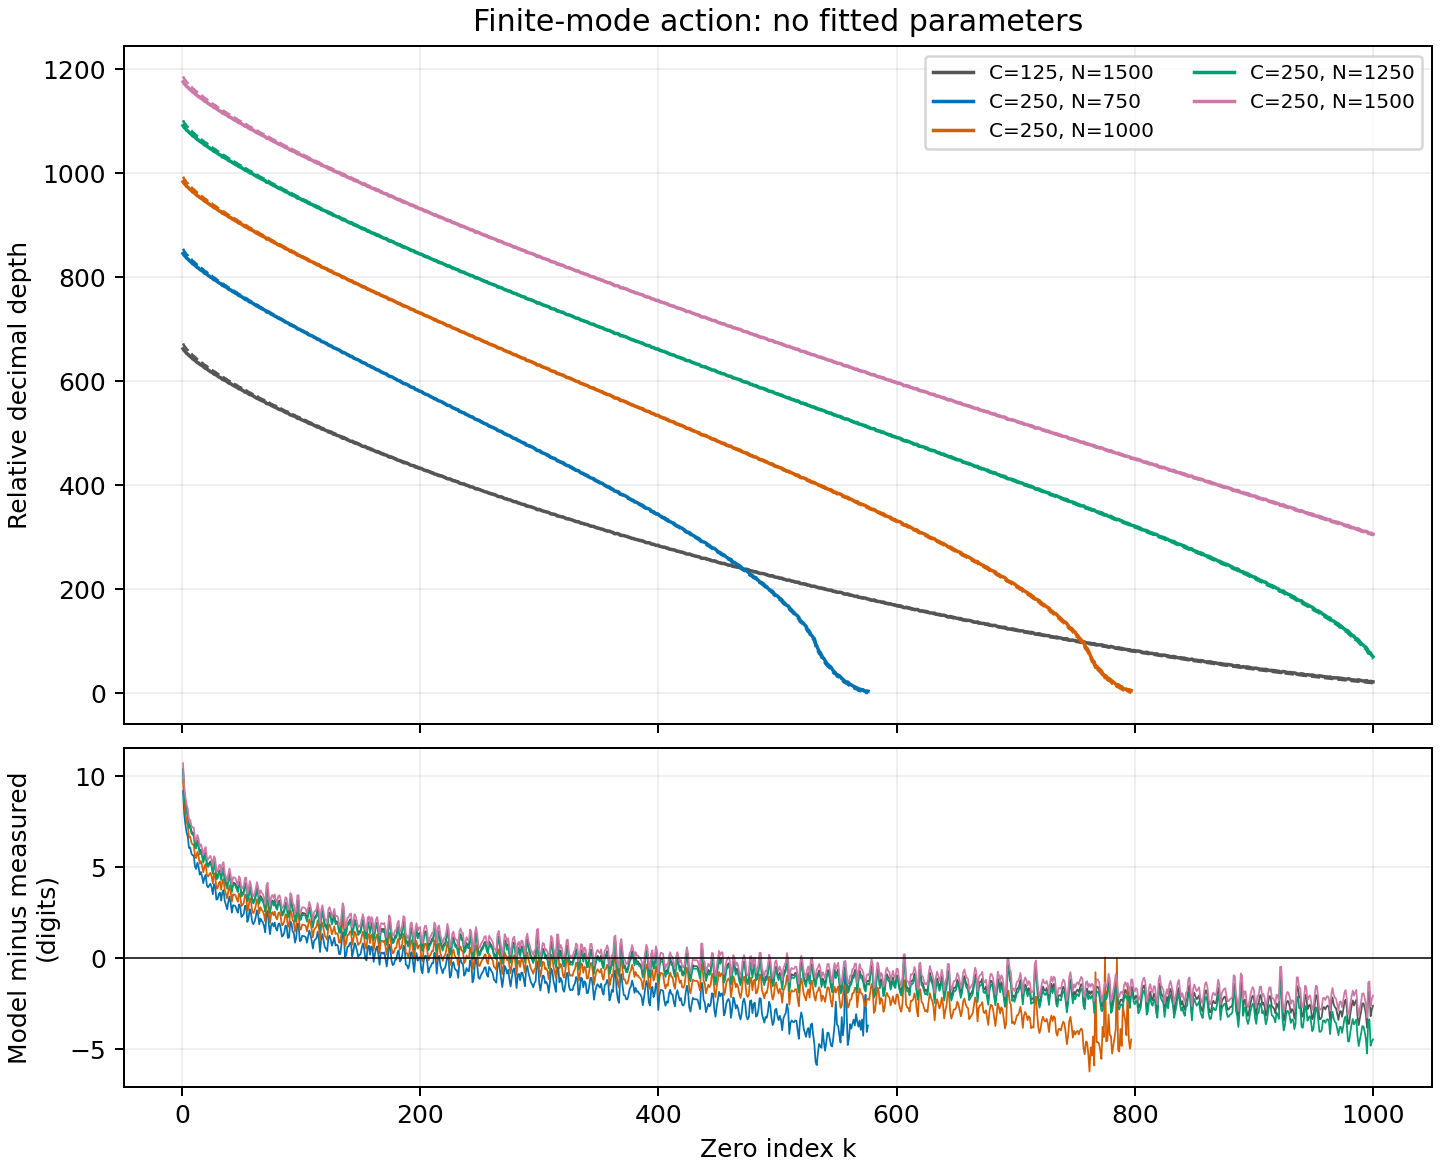
\includegraphics[width=.94\linewidth]{figures/continuum_action.png}
\caption{Measured depths (solid) and the derived continuum-model action
(dashed), with their difference below. Close agreement on a thousand-digit
scale does not establish accurate displacement prediction.}
\label{fig:continuum-action}
\end{figure}
